\documentclass[10pt,a4paper,twocolumn]{article}
\usepackage[spanish,es-nodecimaldot]{babel}
\usepackage[utf8]{inputenc}
\usepackage[T1]{fontenc}
\usepackage{lmodern,microtype}
\usepackage{graphicx,float,subcaption}
\usepackage{amsmath,amssymb,booktabs,tabularx,array}
\usepackage{geometry,caption,siunitx,hyperref}
\geometry{margin=1.8cm}
\setlength{\columnsep}{0.7cm}
\setlength{\parindent}{1em}
\setlength{\parskip}{2pt}
\captionsetup{font=small,labelfont=bf}
\sisetup{output-decimal-marker={.}}
\begin{document}

% ENCABEZADO A UNA COLUMNA
\twocolumn[{
\begin{center}
{\LARGE\bfseries CLASIFICACIÓN DEL ESTADO FETAL MEDIANTE CARDIOTOCOGRAFÍA Y MACHINE LEARNING.\par}
\vspace{0.55em}
{\normalsize Dylan Luisjuan Rico \quad Leonardo Alejandro Ambriz Mendoza \quad Derek Lugo Aguirre \quad Ricardo Chávez Altamirano\par}
\vspace{0.35em}
{\small Centro Universitario de Guadalajara (CUGDL)\\ Universidad de Guadalajara\par}
\end{center}
\vspace{0.4em}
\begin{minipage}{\textwidth}
\begin{center}\textbf{Resumen}\end{center}
Este trabajo estudia el uso de algoritmos de aprendizaje automático para clasificar registros cardiotocográficos (CTG) en tres categorías: normal, sospechoso y patológico. Se implementaron dos métodos de clasificación, K vecinos más cercanos (KNN) y regresión logística multiclase mediante la estrategia uno contra el resto (OvR), tanto con implementaciones propias como con herramientas de \texttt{scikit-learn}. Se describe el preprocesamiento de los datos, la evaluación mediante métricas de clasificación y el análisis empírico de los tiempos de entrenamiento y predicción. Además, se estudia la complejidad temporal de los algoritmos y se comparan sus resultados con las implementaciones de referencia. Los experimentos muestran que KNN obtuvo los mejores resultados globales de clasificación en este conjunto de datos, mientras que las implementaciones optimizadas de \texttt{scikit-learn} presentaron ventajas importantes en el tiempo de predicción de KNN. Los resultados deben interpretarse como una evaluación experimental de clasificación de estados fetales y no como un sistema de diagnóstico clínico autónomo.

\vspace{0.4em}
\noindent\textbf{Palabras clave:} aprendizaje automático, cardiotocografía, KNN, regresión logística, clasificación, complejidad temporal.
\vspace{0.8em}
\end{minipage}
}]

\section{Introducción}
La cardiotocografía (CTG) es una técnica utilizada durante el seguimiento fetal para registrar la frecuencia cardiaca fetal y la actividad uterina. La interpretación de estos registros permite identificar patrones asociados con estados normales o con posibles señales de compromiso fetal (Campos \& Bernardes, 2000). Sin embargo, el análisis puede ser complejo y presentar variabilidad entre observadores, por lo que las técnicas de aprendizaje automático representan una alternativa para apoyar la clasificación de los registros.

El objetivo de este proyecto es implementar y comparar algoritmos de clasificación capaces de identificar tres estados del registro cardiotocográfico: normal, sospechoso y patológico. Para ello se desarrollaron implementaciones propias de K vecinos más cercanos y regresión logística multiclase OvR, y se contrastaron con las implementaciones disponibles en \texttt{scikit-learn}. Además de comparar el desempeño predictivo, se analizaron los tiempos de entrenamiento y predicción conforme aumenta el tamaño de los datos.

\section{Planteamiento del problema}
La identificación oportuna de patrones cardiotocográficos anormales es importante para la vigilancia del bienestar fetal. La clasificación manual de los registros puede ser difícil debido a la cantidad de características que deben analizarse y a la posible ambigüedad de algunos patrones, especialmente en la categoría sospechosa.

El problema abordado consiste en construir modelos que, a partir de las características numéricas de un registro CTG, predigan una de tres clases: normal, sospechoso o patológico. El conjunto de datos empleado contiene 2\,126 registros y 21 características predictoras. La distribución es desigual: aproximadamente 77.85\% normal, 13.88\% sospechoso y 8.28\% patológico (Campos \& Bernardes, 2000). Este desbalance debe considerarse al interpretar las métricas, ya que una exactitud elevada puede ocultar un desempeño menor en las clases minoritarias.

\section{Metodología}
\subsection{Conjunto de datos y preparación}
Se utilizó el archivo \texttt{CTG\_clean.csv}, compuesto por 2\,126 observaciones, 21 variables predictoras y una variable objetivo con tres categorías NSP (Campos \& Bernardes, 2000). Para el experimento de clasificación se utilizó una partición de 80\% para entrenamiento y 20\% para prueba, con semilla aleatoria 42: 1\,701 registros de entrenamiento y 425 de prueba. Las características se estandarizaron mediante puntuaciones Z:
\[
z = \frac{x-\mu_{\mathrm{train}}}{\sigma_{\mathrm{train}}},
\]
donde la media y desviación estándar se calcularon únicamente con los datos de entrenamiento y después se aplicaron al conjunto de prueba para evitar fuga de información (Pedregosa et al., 2011).

El experimento de complejidad temporal se realizó por separado: se generaron diez tamaños de muestra, del 10\% al 100\%, con particiones estratificadas de 80/20. Por ello, los tamaños de entrenamiento y prueba de ese experimento no deben confundirse con los de clasificación. En el tamaño del 100\%, el experimento temporal utilizó 1\,700 registros de entrenamiento y 426 de prueba.

\subsection{K vecinos más cercanos (KNN)}
KNN clasifica una observación nueva mediante las etiquetas de sus $k$ vecinos más cercanos dentro del conjunto de entrenamiento. Se utilizó $k=5$, distancia euclidiana y votación uniforme (Scikit-learn Developers, 2026):
\[
d(x,y)=\sqrt{\sum_{j=1}^{p}(x_j-y_j)^2}.
\]
La distancia euclidiana permite medir la proximidad entre las observaciones en el espacio de características (Scikit-learn Developers, 2026).
En la implementación propia, el entrenamiento conserva los datos de referencia, por lo que su costo adicional de ajuste es $O(1)$ si se considera únicamente almacenar referencias. Para cada una de las $M$ observaciones de prueba, la predicción calcula distancias contra las $N$ observaciones de entrenamiento y ordena las distancias (NumPy Developers, 2026). El costo es:
\[
O\left(M(Np+N\log N)\right).
\]
Con $p$ fijo se simplifica a $O(MN\log N)$. La implementación de \texttt{scikit-learn} utilizó distancia euclidiana, \texttt{algorithm=auto} y \texttt{n\_jobs=-1}. Para el número de características utilizado, el análisis considera búsqueda por fuerza bruta, con costo aproximado de predicción $O(MNp)$ esto se mantiene ya que aun si la vectorizacion y paralelismo ayudan a reducir tiempo practio esto no significa que se elimina el trabajo asintótico. En la implementación propia, el entrenamiento únicamente almacena las referencias de los datos, por lo que su costo adicional es constante: \(O(1)\).

En scikit-learn, el entrenamiento realiza validaciones y preparación de los datos antes de almacenarlos. Por ello, su costo depende del tamaño del conjunto de entrada y puede aproximarse por $O(Np) $. Como las características se mantienen fijas en este experimento (p=21), el crecimiento respecto al número de registros es lineal: $O(N) $. 
Los otros algoritmos como kd tree y ball tree usan $O(pNlogN)$ lo cual solo se mencionara pues no hacen parte de este caso al tener p > 15 se selecciona bruteforce por el auto (Scikit-learn Developers, 2026)..

\subsection{Regresión logística multiclase OvR}
La regresión logística se adaptó al problema de tres clases mediante One-vs-Rest (OvR). Se entrena un clasificador binario por clase y la predicción final corresponde al mayor puntaje (Scikit-learn Developers, 2026). La implementación propia utilizó tasa de aprendizaje 0.1 y 2\,000 iteraciones de descenso de gradiente por lotes. Su complejidad de entrenamiento se aproxima por:
\[
O(CINp),
\]
donde $C$ es el número de clases, $I$ las iteraciones, $N$ las muestras y $p$ las características. Si $C$, $I$ y $p$ son fijos, el costo es $O(N)$. La predicción requiere:
\[
O(CMp),
\]
que con $C$ y $p$ fijos se simplifica a $O(M)$.

La versión de referencia utilizó \texttt{OneVsRestClassifier} y \texttt{LogisticRegression(solver=lbfgs, max\_iter=2000, random\_state=42)}. L-BFGS determina las iteraciones según convergencia y tolerancia, con un máximo de 2\,000. Su costo de entrenamiento se aproxima como $O(CI_{\mathrm{LBFGS}}Np)$ y el de predicción como $O(CMp)$ (Scikit-learn Developers, 2026).

\subsection{Evaluación y medición}
El desempeño se evaluó mediante Accuracy, F1 macro y Recall por clase. F1 macro promedia sin ponderación el F1 de cada categoría, dando igual importancia a las clases minoritarias. El Recall por clase permite observar la proporción de casos reales de cada categoría identificados correctamente (Pedregosa et al., 2011).

Para el análisis temporal se utilizaron diez fracciones del conjunto de datos, del 10\% al 100\%. Se midieron por separado los tiempos de ajuste (\textit{fit}) y predicción (\textit{predict}) mediante \texttt{time.perf\_counter()}. Se descartó un calentamiento inicial y se ejecutaron siete repeticiones por configuración. Se reportan medianas en milisegundos. Se ajustaron curvas y se calculó $R^2$. Un $R^2$ alto respalda el ajuste empírico en el intervalo medido, pero no demuestra matemáticamente la complejidad asintótica. Los tiempos dependen también del hardware, versiones de bibliotecas, carga del sistema y paralelismo.

\section{Resultados}
\subsection{Desempeño de clasificación}
La Tabla~\ref{tab:clasificacion} resume las métricas globales. KNN presentó la mayor exactitud y F1 macro; las diferencias entre implementaciones propias y \texttt{scikit-learn} fueron pequeñas.

\begin{table}[H]
\centering
\caption{Métricas globales de clasificación.}
\label{tab:clasificacion}
\small
\begin{tabular}{lcc}
\toprule
\textbf{Modelo} & \textbf{Accuracy} & \textbf{F1 macro}\\
\midrule
KNN propio & 90.12\% & 81.64\%\\
KNN scikit-learn & 89.88\% & 80.77\%\\
OvR propio & 87.76\% & 76.72\%\\
OvR scikit-learn & 87.29\% & 76.59\%\\
\bottomrule
\end{tabular}
\end{table}

\begin{table}[H]
\centering
\caption{Recall por clase.}
\label{tab:recall}
\small
\begin{tabular}{lccc}
\toprule
\textbf{Modelo} & \textbf{Normal} & \textbf{Sospechoso} & \textbf{Patológico}\\
\midrule
KNN propio & 97.28\% & 61.02\% & 71.43\%\\
KNN scikit-learn & 97.28\% & 61.02\% & 68.57\%\\
OvR propio & 95.77\% & 52.54\% & 71.43\%\\
OvR scikit-learn & 94.86\% & 52.54\% & 74.29\%\\
\bottomrule
\end{tabular}
\end{table}

La categoría sospechosa presentó los valores de Recall más bajos para todos los modelos. KNN propio obtuvo el mejor equilibrio global según Accuracy y F1 macro. La regresión logística de \texttt{scikit-learn} tuvo Recall de 74.29\% en la clase patológica, ligeramente superior al de la versión propia.

\subsection{Tiempos de entrenamiento}
La Tabla~\ref{tab:fit} presenta las medianas de entrenamiento para tres tamaños representativos. KNN propio tiene un tiempo de ajuste mínimo porque conserva los datos sin optimización iterativa; la regresión logística propia ejecuta las iteraciones del descenso de gradiente. La implementación de \texttt{scikit-learn} reduce notablemente este tiempo (Pedregosa et al., 2011).

\begin{table}[H]
\centering
\caption{Mediana del tiempo de entrenamiento (ms).}
\label{tab:fit}
\scriptsize
\begin{tabular}{crrrr}
\toprule
\textbf{Fracción} & \textbf{KNN P.} & \textbf{KNN SK} & \textbf{OvR P.} & \textbf{OvR SK}\\
\midrule
10\% & 0.0010 & 0.6999 & 115.8238 & 22.4092\\
50\% & 0.0010 & 0.7603 & 203.4343 & 29.9500\\
100\% & 0.0010 & 0.8375 & 320.7521 & 42.7461\\
\bottomrule
\end{tabular}
\end{table}

% GRAFICA DE TIEMPOS DE ENTRENAMIENTO AQUI
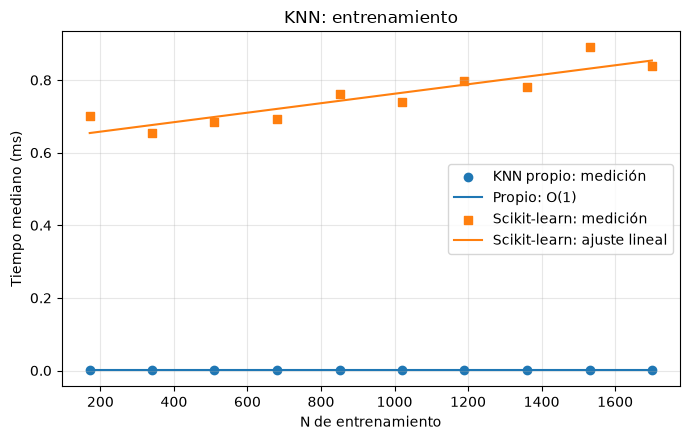
\includegraphics[width=\columnwidth]{KNN_entrenamiento.png}
\begin{figure}[H]
\centering
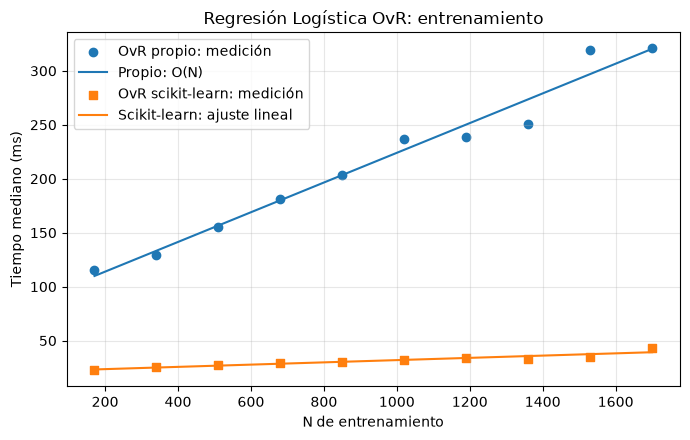
\includegraphics[width=\columnwidth]{RegresionLogisticaOvR_entrenamiento.png}
\caption{Comparación de los tiempos de entrenamiento conforme aumenta el tamaño del conjunto de datos.}
\label{fig:tiempos-fit}
\end{figure}

La Figura 1 permite observar cómo cambian los tiempos de entrenamiento de las cuatro implementaciones conforme aumenta el tamaño de la muestra.

\subsection{Tiempos de predicción}
La Tabla~\ref{tab:predict} presenta los tiempos de predicción. En KNN propio, el costo aumenta considerablemente con el tamaño del conjunto de entrenamiento debido al cálculo y ordenamiento de distancias. La implementación de \texttt{scikit-learn} reduce notablemente este tiempo.

\begin{table}[H]
\centering
\caption{Mediana del tiempo de predicción (ms).}
\label{tab:predict}
\scriptsize
\begin{tabular}{crrrr}
\toprule
\textbf{Fracción} & \textbf{KNN P.} & \textbf{KNN SK} & \textbf{OvR P.} & \textbf{OvR SK}\\
\midrule
10\% & 31.9714 & 3.9090 & 0.0542 & 0.5341\\
50\% & 692.6658 & 7.2958 & 0.0653 & 0.5137\\
100\% & 2926.5604 & 3.7136 & 0.0819 & 0.6229\\
\bottomrule
\end{tabular}
\end{table}

%GRAFICA DE TIEMPOS DE PREDICCION AQUI 
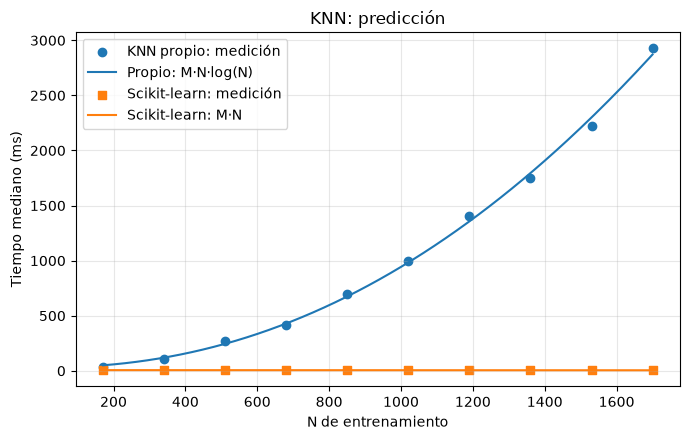
\includegraphics[width=\columnwidth]{KNN_prediccion.png}
\begin{figure}[H]
\centering
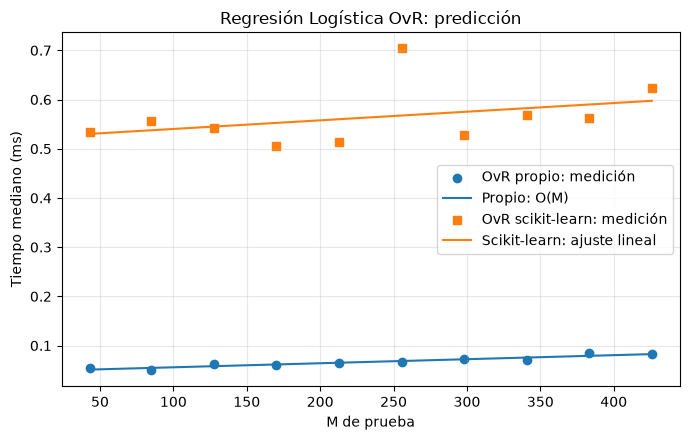
\includegraphics[width=\columnwidth]{RegresionLogisticaOvR_prediccion.png}
\caption{Comparación de los tiempos de predicción conforme aumenta el tamaño del conjunto de datos.}
\label{fig:tiempos-predict}
\end{figure}

La Figura 2 muestra las diferencias en los tiempos de predicción, destacando el crecimiento del KNN propio frente a las implementaciones de scikit-learn.

\subsection{Ajuste de las curvas temporales}
\begin{table}[H]
\centering
\caption{Coeficiente de determinación $R^2$ de los ajustes temporales.}
\label{tab:r2}
\small
\begin{tabular}{lcc}
\toprule
\textbf{Modelo} & \textbf{Fit} & \textbf{Predict}\\
\midrule
KNN propio & 0.0000 & 0.9982\\
KNN scikit-learn & 0.8189 & 0.0445\\
OvR propio & 0.9729 & 0.8926\\
OvR scikit-learn & 0.9070 & 0.1453\\
\bottomrule
\end{tabular}
\end{table}

Los valores altos de $R^2$ para predicción de KNN propio y para ajuste y predicción de OvR propio indican que las curvas describen razonablemente los datos observados. Los valores bajos de KNN scikit-learn y de predicción de OvR scikit-learn indican que, en el intervalo medido, los tiempos no siguen claramente la curva ajustada. Esto no invalida el análisis asintótico; refleja que el ajuste empírico no explica bien esas mediciones concretas.

\section{Discusión}
KNN alcanzó el mejor desempeño global de clasificación. La diferencia entre su implementación propia y la de \texttt{scikit-learn} fue reducida en Accuracy y F1 macro. Sin embargo, el Recall de la clase sospechosa fue menor para todos los modelos, por lo que esta categoría representa el principal reto de clasificación.

El análisis temporal mostró una diferencia importante entre el costo de entrenamiento y el de predicción de KNN. La implementación propia tiene un ajuste prácticamente constante, pero su predicción es costosa al calcular y ordenar distancias para cada caso. La versión de \texttt{scikit-learn} mostró tiempos de predicción considerablemente menores, debido a sus rutinas optimizadas.

Para regresión logística, el entrenamiento de la implementación propia fue más lento que el de \texttt{scikit-learn} en los tamaños representativos. Esto es consistente con el uso de L-BFGS frente a un número fijo de iteraciones de descenso de gradiente. En predicción, ambas implementaciones mantuvieron tiempos bajos frente a KNN propio.

Las tendencias experimentales son compatibles con las expresiones de complejidad presentadas, aunque los ajustes empíricos no sustituyen el análisis teórico. Los tiempos también dependen del entorno de ejecución. Finalmente, el sistema clasifica registros CTG en categorías NSP; no predice directamente la mortalidad fetal ni sustituye la valoración de profesionales de la salud. Cualquier posible uso como herramienta de apoyo requeriría validación clínica y pruebas con datos independientes.

\section{Conclusiones}
Se implementaron y compararon KNN y regresión logística OvR mediante versiones propias y versiones de \texttt{scikit-learn}. KNN obtuvo los mejores resultados globales, con 90.12\% de Accuracy y 81.64\% de F1 macro en su implementación propia.

El análisis temporal mostró que KNN propio tiene un costo de entrenamiento mínimo, pero un costo de predicción elevado al crecer el conjunto de entrenamiento. La versión de \texttt{scikit-learn} fue considerablemente más rápida en predicción. En regresión logística, la implementación propia presentó mayor tiempo de entrenamiento que la versión basada en L-BFGS. Los resultados son experimentales y no deben interpretarse como evidencia de diagnóstico o predicción directa de mortalidad fetal.

\section{Bibliografia}

\begingroup
\setlength{\parindent}{0pt}
\setlength{\parskip}{6pt}

\noindent\hangindent=1.27cm\hangafter=1
Campos, D., y Bernardes, J. (2000). \textit{Cardiotocography} [Conjunto de datos]. UCI Machine Learning Repository. \url{https://doi.org/10.24432/C51S4N}

\noindent\hangindent=1.27cm\hangafter=1
NumPy Developers. (2026). \textit{numpy.argsort} (Versión 2.5) [Documentación de software]. \url{https://numpy.org}

\noindent\hangindent=1.27cm\hangafter=1
Pedregosa, F., Varoquaux, G., Gramfort, A., Michel, V., Thirion, B., Grisel, O., Blondel, M., Prettenhofer, P., Weiss, R., Dubourg, V., Vanderplas, J., Passos, A., Cournapeau, D., Brucher, M., Perrot, M., y Duchesnay, É. (2011). Scikit-learn: Machine learning in Python. \textit{Journal of Machine Learning Research}, \textit{12}, 2825–2830. \url{https://jmlr.org}

\noindent\hangindent=1.27cm\hangafter=1
Scikit-learn Developers. (2026). \textit{LogisticRegression} (Versión 1.9.1) [Documentación de software]. \url{https://scikit-learn.org}

\noindent\hangindent=1.27cm\hangafter=1
Scikit-learn Developers. (2026). \textit{Nearest Neighbors} (Versión 1.9.1) [Documentación de software]. \url{https://scikit-learn.org}


\end{document}
